\section{Design}

Given the scope of the practical, simplicity was the main goal when considering the design of the RDT protocol. This section will discuss the design decisions and rationale behind them. The two attempted extension features, checksums and adaptive re-transmission timeouts,  are also detailed here.

\subsection{Packet Structure}

RDT packets (see Figure~\ref{fig:packet}) are composed of a constant 12 byte header and an optional data segment. The size of the data segment ranges from 0 to 1300 bytes, with 1300 bytes used as the maximum size so as not to interfere with the operation of \code{slurpe-3}, which was used for testing. \textbf{Theoretical maximum size?}.

\begin{figure}[h]
\begin{verbatim}
+-+-+-+-+-+-+-+-+-+-+-+-+-+-+-+-+-+-+-+-+-+-+-+-+-+-+-+-+-+-+-+-+
|   Header (12 Bytes)   |         Data (0 - 1300 Bytes)         |
+-+-+-+-+-+-+-+-+-+-+-+-+-+-+-+-+-+-+-+-+-+-+-+-+-+-+-+-+-+-+-+-+
\end{verbatim}
\caption{RDT Packet Structure}\label{fig:packet}
\end{figure}

The RDT header (see Figure~\ref{fig:header}) is comprised of the following fields: a 32-bit \code{sequence} field, used for \textbf{what?}; a 16-bit \code{type} field, used to denote the packet function (see Figure); a 16-bit \code{checksum} field, calculated over the header and data segment to \textbf{what?}; a 16-bit \code{size} field denoting the size of the data segment (in bytes); and a 16-bit \code{padding} field to ensure 32-bit word alignment.

Several factors influenced the RDT header design. As the \textbf{C library function} \code{ftell} (used to calculating file sizes in \code{RdtClient.c}) returns 32-bit \code{long} values, a 32-bit \code{sequence} field was required to support the transmission of large files/amounts of data. The given implentation of the IPv4 header checksum used returns a \code{uint16\char`_t} value, thus necessitating a 16-bit field. As a maximum data segment size of 1300 bytes was required, at least 11 bits were required for the \code{size} field, however 16 bits were used for alignment. For the remaining \code{type} and \code{padding} fields, there were no other considerations for field size other than 32-bit alignment. 

\begin{figure}
\begin{center}
\begin{verbatim}
 0                   1                   2                   3  
 0 1 2 3 4 5 6 7 8 9 0 1 2 3 4 5 6 7 8 9 0 1 2 3 4 5 6 7 8 9 0 1
+-+-+-+-+-+-+-+-+-+-+-+-+-+-+-+-+-+-+-+-+-+-+-+-+-+-+-+-+-+-+-+-+
|                            Sequence                           |
+-+-+-+-+-+-+-+-+-+-+-+-+-+-+-+-+-+-+-+-+-+-+-+-+-+-+-+-+-+-+-+-+
|              Type             |            Checksum           |
+-+-+-+-+-+-+-+-+-+-+-+-+-+-+-+-+-+-+-+-+-+-+-+-+-+-+-+-+-+-+-+-+
|              Size             |            Padding            |
+-+-+-+-+-+-+-+-+-+-+-+-+-+-+-+-+-+-+-+-+-+-+-+-+-+-+-+-+-+-+-+-+
\end{verbatim}
\end{center}
\caption{RDT Header}\label{fig:header}
\end{figure}

A single type field was chosen, rather than a set TCP-style flags, for simplicity. Given the minimal nature of the RDT protocol, it was faster simpler to enumerate all packet types (see Figure), rather than testing multiple flags.

The type field supports the following types: \code{SYN} (0) and \code{SYN ACK} (1), used for the connection handshake; \code{DATA} (2) and \code{ACK} (3), used for sending and acknowledging data segments; \code{FIN} (4) and \code{FIN ACK} (5), used for graceful connection termination; and \code{RST} (6), used for abrupt connection termination.

\subsection{Connection Management}

The operation of the RDT protocol can be modelled by the FSM in Figure \ref{fig:fsm}. For connection management, a two-way handshake is used. As RDT only supports uni-directional communication, a two-way handshake (see Figure ) is adequate for establishing and terminating connections. Adaptive re-transmission timeouts are used in both the handshakes and transmission of data segments.

\begin{figure}[H]
\begin{center}
    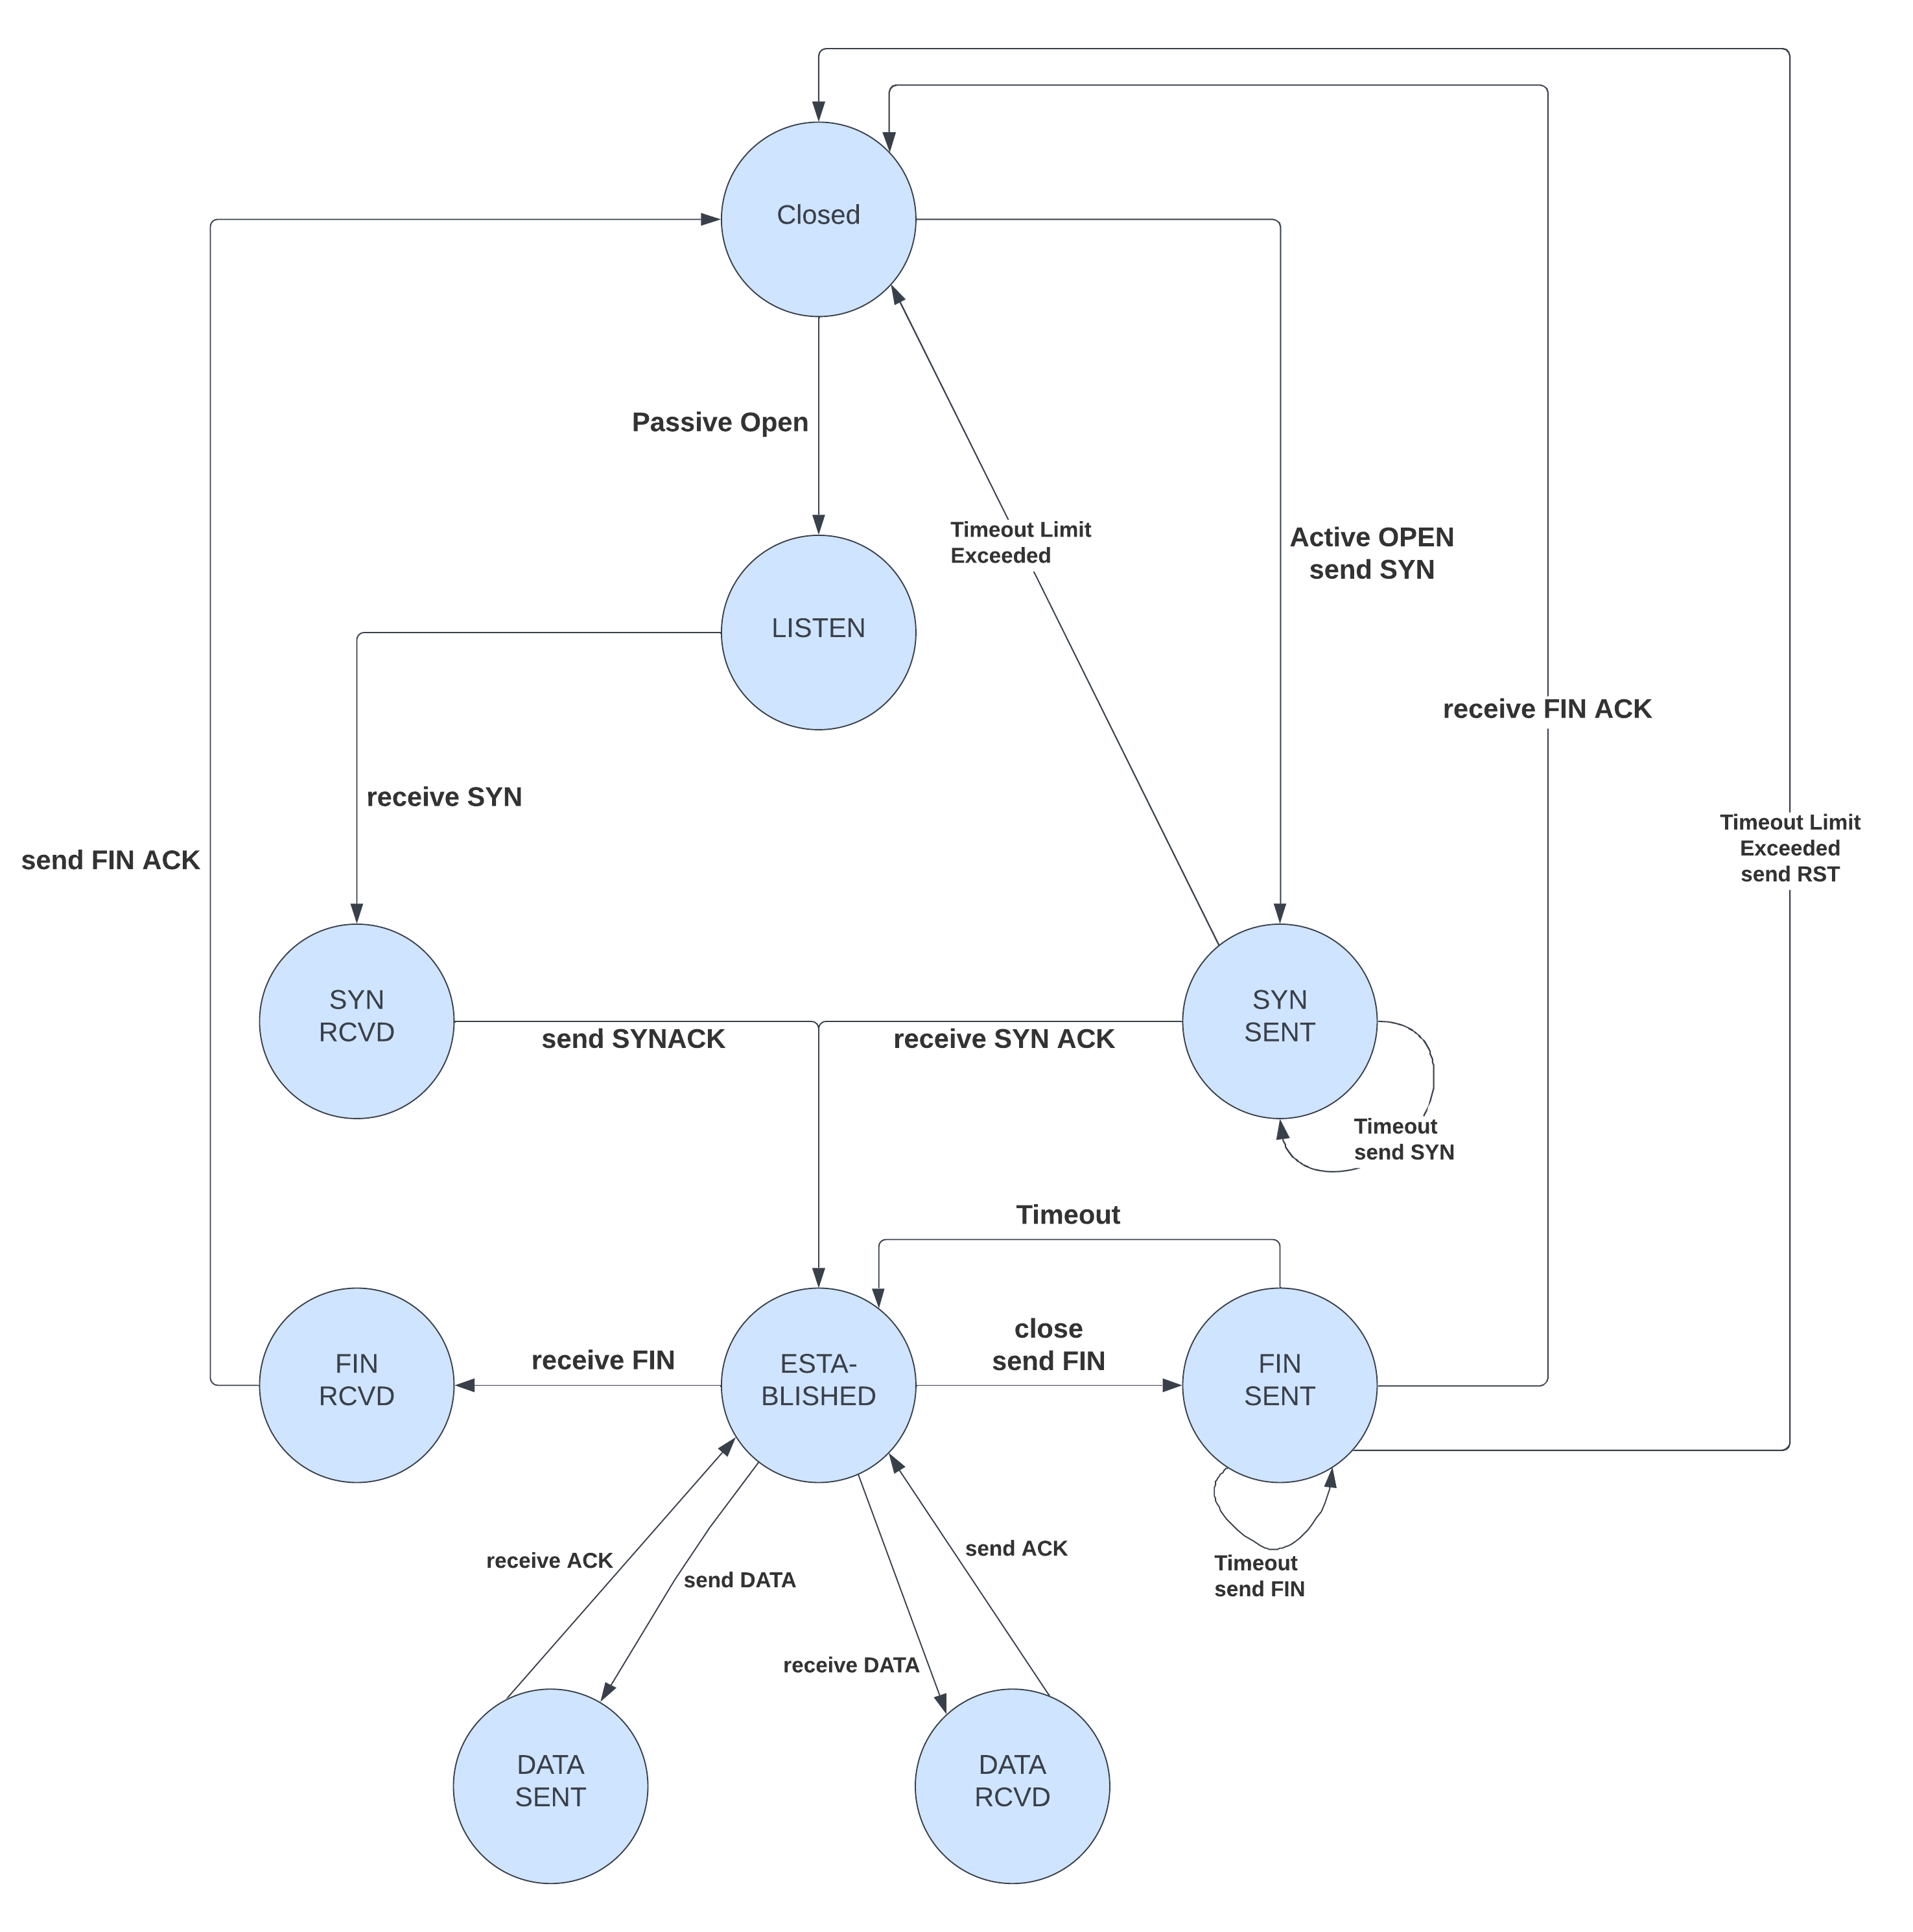
\includegraphics[width=100mm]{images/fsm.png}
\end{center}
\caption{RDT Finite State Machine (see also A.1)}\label{fig:fsm}
\end{figure}

An initial RTO value of 200ms is used for hanshakes, and this doubles until 5 attempts have been made before the connection is abruptly terminated with an \code{RST}.

\begin{figure}[H]
\begin{center}
    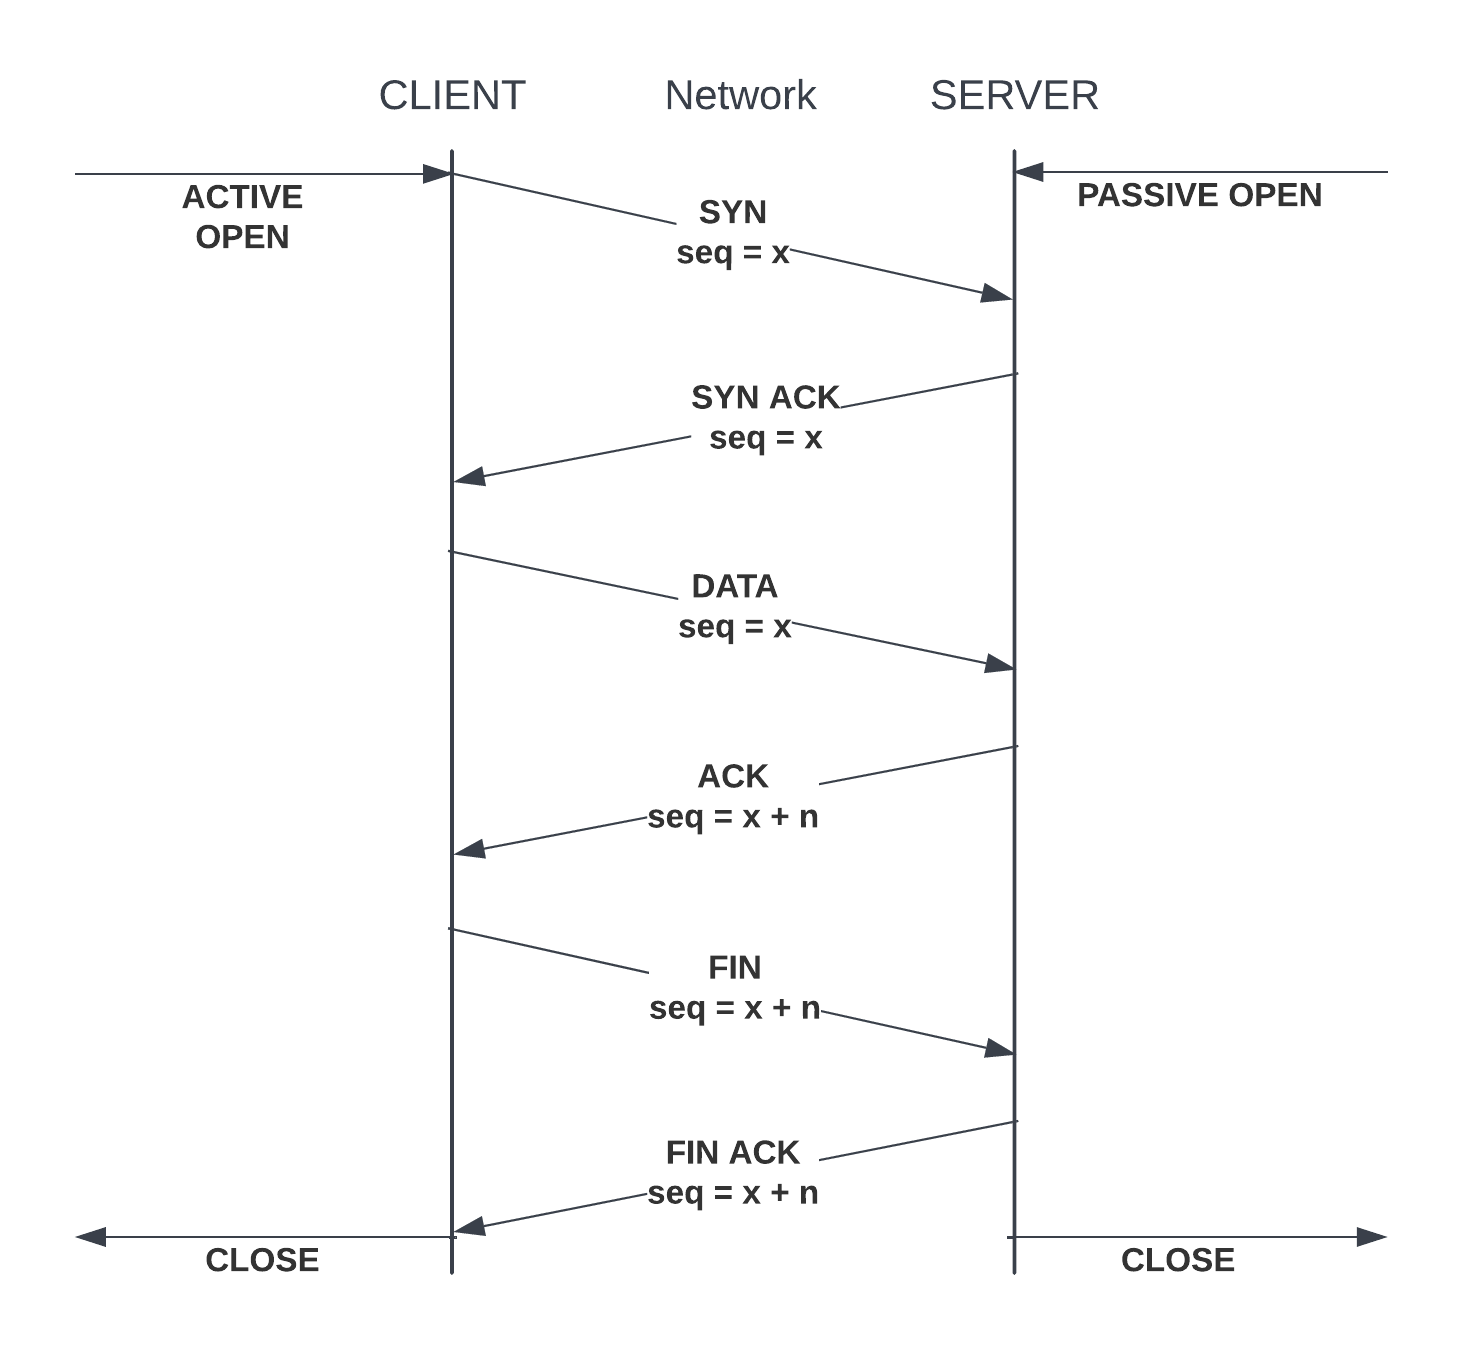
\includegraphics[width=100mm]{images/timeline.png}
\end{center}
\caption{Connection Timeline Diagram (see also A.2)}\label{fig:timeline}
\end{figure}
    

\subsection{Adaptive RTO}
In an extension to the base specification, adaptive re-transmission timeouts using measured RTT has been implemented. RDT's adaptive RDT is modelled on TCP's Retranmission Timer \cite{rfc6298} \footnote{Clock granularity is not considered, however RTO values are calculated in microseconds and the School Lab PCs have a granularity of 1 nanosecond.}. RDT uses the same initial RTO of 1s and maximum of 60s. 


\subsection{Checksum}
The RDT \code{checksum} field is calculated over the entire segment/packet (i.e. header and data) using the IPv4 Header Checksum Algorithm \cite{rfc791}. The implementation of the original source \cite{ipv4_checksum} to support the use of 8-bit byte values in the data segment. During checksum calculating, the \code{checksum} field itself is set to 0 for consistency.